\section{\textit{Stream Processing}}

Secara umum, \textit{stream} merujuk pada data yang tersedia secara inkremental dari waktu ke waktu. Konsep ini dipakai di berbagai tempat, seperti stdin dan stdout Unix, TCP \textit{connection}, dan lain-lain \parencite{dataIntensiveApplications}.

\textit{Stream processing} merupakan paradigma pemrograman yang memandang \textit{streams} atau urutan \textit{events} sebagai objek \textit{input} dan \textit{output} utama dari komputasi. \cite{streaming101} menyatakan bahwa \textit{stream processing} merupakan tipe \textit{engine} pemrosesan data yang didesain dengan mempertimbangkan \textit{dataset} yang tidak terbatas.

\cite{streamProcessingComparison} menyatakan bahwa terdapat karakteristik penting pada \textit{stream processing}, yaitu:

\begin{enumerate}
    \item \textit{Delivery guarantees}. Setiap informasi yang masuk harus dijamin akan diproses oleh \textit{streaming engine}.
    \item \textit{Fault tolerance}. Ketika terjadi kegagalan, \textit{streaming engine} harus mampu melakukan \textit{recovery} dan memulai ulang dari titik yang ditinggalkan.
    \item \textit{State management}. \textit{Streaming engine} harus memiliki mekanisme untuk menyimpan dan memperbarui informasi \textit{state}.
    \item Memiliki kinerja yang baik dari sisi latensi, \textit{throughput}, dan \textit{scalability}.
    \item Memiliki fitur yang lebih \textit{advances}, seperti \textit{event time processing}, \textit{watermarks}, \textit{windowing}, dan lain-lain.
\end{enumerate}

Selain itu, karakteristik \textit{stream processing} juga bisa dibagi menjadi dua jenis, yaitu:

\begin{enumerate}
    \item \textit{Native streaming}. \textit{Stream processing} jenis ini akan langsung memproses \textit{record} yang diterima secepat mungkin. Contoh \textit{stream processing} tipe ini adalah Apache Storm, Apache Flink, Apache Kafka Streams, dan Apache Samza.
    \item \textit{Micro-batching}. \textit{Stream processing} jenis ini meproses \textit{record} setiap beberapa detik atau milidetik sekali sehingga \textit{record} diproses dalam setiap \textit{mini-batch} dengan sedikit \textit{delay}. Contoh \textit{stream processing} tipe ini adalah Apahe Spark Streaming dan Apache Storm-Trident.
\end{enumerate}

\subsection{RisingWave}

RisingWave merupakan \textit{cloud-native streaming database}. Setelah menghubungkan sumber \textit{stream}, pengguna dapat membuat kueri analisis dengan mendefinisikan \textit{materialized view}, yang diperbarui secara inkremental pada RisingWave \textit{streaming engine} \parencite{risingwave}.

Berikut adalah keuntungan RisingWave:

\begin{enumerate}
    \item Mudah dipelajari karena merupakan ekstensi dari sintaks PostgreSQL.
    \item Mudah dioperasikan dan memiliki kebutuhan sumber daya yang lebih rendah karena ditulis dalam bahasa sistem Rust.
    \item Mendukung berbagai sumber data dan mampu mengirimkan (\textit{sink}) data ke dalam berbagai sumber, seperti mengambil data dari Apache Kafka lalu hasilnya dikirim ke ClickHouse. RisingWave mendukung integrasi dengan PostgreSQL CDC dan Apache Kafka sebagai sumber (\textit{source}) dan tujuan data (\textit{sink}).
    \item Menjamin konsistensi pada \textit{materialized view} dengan menggunakan \textit{snapshot}.
\end{enumerate}

\begin{figure}[ht]
    \centering
    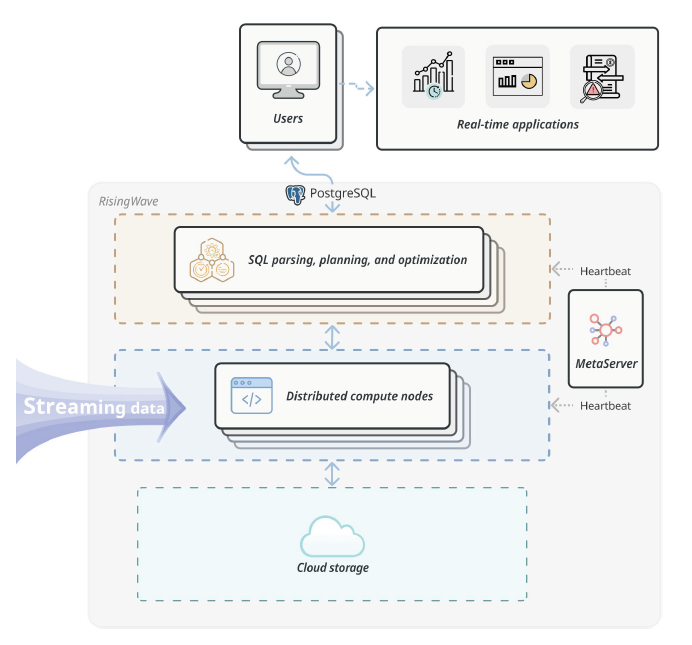
\includegraphics[width=0.8\textwidth]{resources/chapter-2/risingwave.png}
    \caption{Arsitektur RisingWave \parencite{risingwave}}
    \label{fig:risingwave-architecture}
\end{figure}

Node komputasi pada RisingWave terdiri atas \textit{batch engine} dan \textit{streaming engine}. \textit{Batch engine} meliputi \textit{query execution engine} dan \textit{exchange service} untuk menukar data antar node komputasi. \textit{Streaming engine} dibangun atas model aktor pada pemrograman konkuren. Mesin ini berinteraksi langsung dengan \textit{frontend} dan melayani \textit{stream data}. Selain itu, terdapat \textit{meta service} yang berperan sebagai layanan sentral untuk menyimpan metadata seperti keadaan kluster, katalog sistem, keanggotaan kluster, dan lain-lain \parencite{risingwave}.